\documentclass{article}
\usepackage{amsthm}
\usepackage{amsmath}
\usepackage{graphicx}
\usepackage{multirow}
\usepackage{tikz}
\usepackage{wasysym}
\newtheorem{problem}{Problem}

\begin{document}
\title{Exam 2}
\author{Henry Z. Lo}
\maketitle

In this exam, you will be presented with various problems which can be solved by minor variations of the algorithms you have been learning.  You should describe the technique you use to solve the problem, as well as any modifications needed.  

For each problem, do the following in class:

\begin{enumerate}
\item Describe why your solution works (40\%):
\item Provide pseudocode (40\%).
\item Give the runtime for your algorithm, and explain (20\%).
\end{enumerate}

The most important things are that your algorithm is correct and that you have an optimal runtime.  You should give convincing arguments about how and why your algorithms work, so that I can understand your train of thought.

For extra credit, you can program the solutions for each of these problems.  Instructions for this will be given elsewhere.

\pagebreak

\begin{problem}
You promised to provide each home in a small town with running water in our campaign for mayor.  Now you are elected, and you need to give everyone access to water.  It costs $w_i$ to construct a well at house $i$.  For each pair of houses $i$ and $j$, it costs $c_{ij}$ to connect a water pipe between them.  What is the lowest possible cost to the city?
\end{problem}

You will need at least one well to provide everyone with water.

As an example, consider a town with four homes, with the cost matrix:
\begin{center}
\begin{tabular}{|c|cccc|}
\hline
  & A & B & C & D \\
\hline
A & 0 & 5 & 5 & 6 \\
B & 5 & 0 & 3 & 4 \\
C & 5 & 3 & 0 & 6 \\
D & 6 & 4 & 6 & 0 \\
\hline
\end{tabular}
\end{center}

Also, suppose that the cost to build a well at each home is:
\begin{center}
\begin{tabular}{|cccc|}
\hline
A & B & C & D \\
\hline
6 & 7 & 5 & 3 \\
\hline
\end{tabular}
\end{center}

Then the lowest possible cost is to build a well at D, connect it to B, connect B to C, and connect C to A.  This gives a total cost of 15.

You can safely assume that the cost to build a pipe from A to B is the same as the cost from B to A.

\begin{problem}
Given a directed acyclic graph, return a Hamiltonian path if there is one.  Otherwise, return null.  Recall that a Hamiltonian path is a path which visits every vertex exactly once.
\end{problem}

For example, in the following graph, the path $e \rightarrow d \rightarrow c \rightarrow b$ is Hamiltonian.
\begin{center}
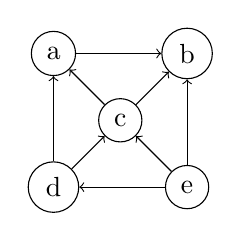
\begin{tikzpicture}[->, node distance=1.2cm, main node/.style={draw,circle}]
\node[main node]                   (c) {c};
\node[main node, above left of=c]  (a) {a};
\node[main node, above right of=c] (b) {b};
\node[main node, below left of=c]  (d) {d};
\node[main node, below right of=c] (e) {e};
\path
(c) edge node {} (a)
    edge node {} (b)
(a) edge node {} (b)
(d) edge node {} (c)
    edge node {} (a)
(e) edge node {} (d)
edge node {} (c)
edge node {} (b)
;
\end{tikzpicture}
\end{center}
You should return this path.  Note that not all directed acyclic graphs have Hamiltonian paths - you will need to detect this.

\begin{problem}
As a network engineer, your first task is to identify the vulnerabilities in the computer network.  Specifically, you want to find all the connections such that if the connection were lost, the network is split into two distinct groups.
\end{problem}

Consider for an example if you had the following network of 6 computers.

\begin{center}
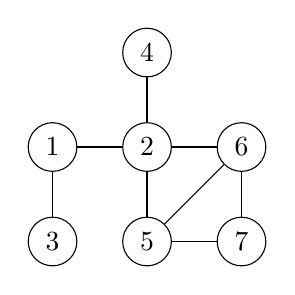
\begin{tikzpicture}[node distance=1.2cm, main node/.style={draw,circle}]
\node[main node]             (1) {1};
\node[main node, right of=1] (2) {2};
\node[main node, below of=1] (3) {3};
\node[main node, above of=2] (4) {4};
\node[main node, below of=2] (5) {5};
\node[main node, right of=2] (6) {6};
\node[main node, below of=6] (7) {7};
\path
(1) edge node {} (2)
    edge node {} (3)
(2) edge node {} (4)
    edge node {} (5)
(6) edge node {} (2)
    edge node {} (5)
    edge node {} (7)
(5) edge node {} (7);
\end{tikzpicture}
\end{center}

Here, if the connections between 2 and 6 were to break, then they are still connected via 5, and via 5 and 7.  Contrast this with 1 and 3.  If the edge between 1 and 2 broke, then 1 and 3 would be isolated.  Likewise with 4.  These are the edges we are looking for.

The edge set you should return for this graph is 1$\rightarrow$2, 1$\rightarrow$3, and 2$\rightarrow$4.  Assume the graph is undirected.

\begin{problem}
Given a set of currencies, and their exchange rates to each other, find the most maximum amount of $c_j$ you can get for one $c_i$.  Exchange rates are directed.
\end{problem}

For example, consider the exchange rates below.

\begin{center}
\begin{tabular}{|c|c|}
\hline
From & To \\
\hline
\multirow{3}{*}{1 Dollar} & 0.75 Euros \\
& 100 Yen \\
& 0.5 Pounds \\
\hline
\multirow{2}{*}{1 Euro} & 125 Yen \\
& 0.8 Pounds \\
& 1.2 Dollars \\
\hline
1 Yen & 0.0065 Pounds \\
& .009 Dollars \\
\hline
\end{tabular}
\end{center}

If we want to exchange one dollar to pounds, we can do so directly for half a pound, or we can first convert to 100 yen, then to 0.7 pounds.  This is the most we can get for this exchange, so this is the correct answer.

You can safely assume that there are no cycles in which you can make money infinitely (your broker takes a bit from each exchange).

\end{document}

